\chapter{Background Research}
\label{chap:research}

At the start of our project, we conducted background research on terms,
concepts, and conditions mentioned by our client, Dr. Kate Enzler from the
Alexian Rehab Hospital, in her request for a design for something to alleviate
left neglect. Left neglect is a neurological condition wherein patients have
decreased response to their left sides, a condition our team has no background
on. Our background research helped us understand left neglect, its severity,
and current solutions to give us foundational knowledge needed for creating an
effective design. This research was separated into three main sections: (1)
defining left neglect, (2) understanding struggles patients with left neglect
face, and (3) reviewing current approaches to left neglect. 

\section{Defining left neglect}

Left neglect is a type of unilateral spatial neglect (USN), a syndrome that
occurs after brain hemisphere damage [1]. Literature suggests that left neglect
is more severe than right neglect [1], as well as 71\% more frequent[2]. While
left and right USN are both common after stroke [1], this higher frequency
makes it more important to address left neglect due to its prevalence.

Literature also suggests that certain deficiencies are more severe for patients
with left neglect. Peripersonal and extrapersonal neglect (neglect of one’s
personal space and neglect of one’s immediate surroundings respectively) were
found to be more frequent for patients with left neglect [1]. While right
neglect also leads to deficiencies such as poorer balance [1], these
left-dsided deficiencies highlight the need for something to alleviate left
neglect. \autoref{fig:processing} depicts the difference in brain response to
stimuli for patients with no USN, right USN, and left USN.

\begin{figure}[h]
  \centering
  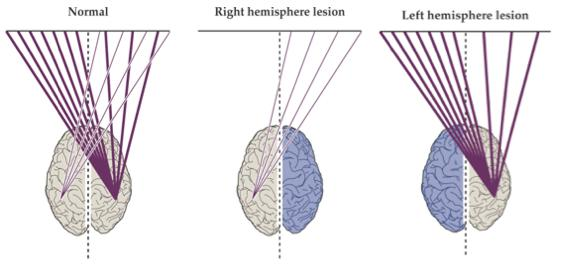
\includegraphics[width=0.5\textwidth]{processing}
  \caption[Environment processing in the brain.]{Diagram illustrating the
    effect of both left and right unilateral spatial neglect on neurological
    response to stimuli on both sides of the brain [2]. Here, right neglect is
    shown to eliminate left-side brain interactions while left neglect still
    has some interaction with both sides. This implies that right neglect is
    more severe, making it substantially more difficult to address than left
    neglect. This key difference also implies that a solution to left or right
    neglect is not a universal solution to unilateral spatial neglect; such a
    universal solution would require further research, planning, and
    resources.}
  \label{fig:processing}
\end{figure}

\section{Understanding struggles patients with left neglect face}

Patients experiencing left neglect have a reduced ability to interact with the
left side of their perceived world. \autoref{fig:fov}, below, compares the
interactions of patients with USN to patients without USN. 

\begin{figure}[h]
  \centering
  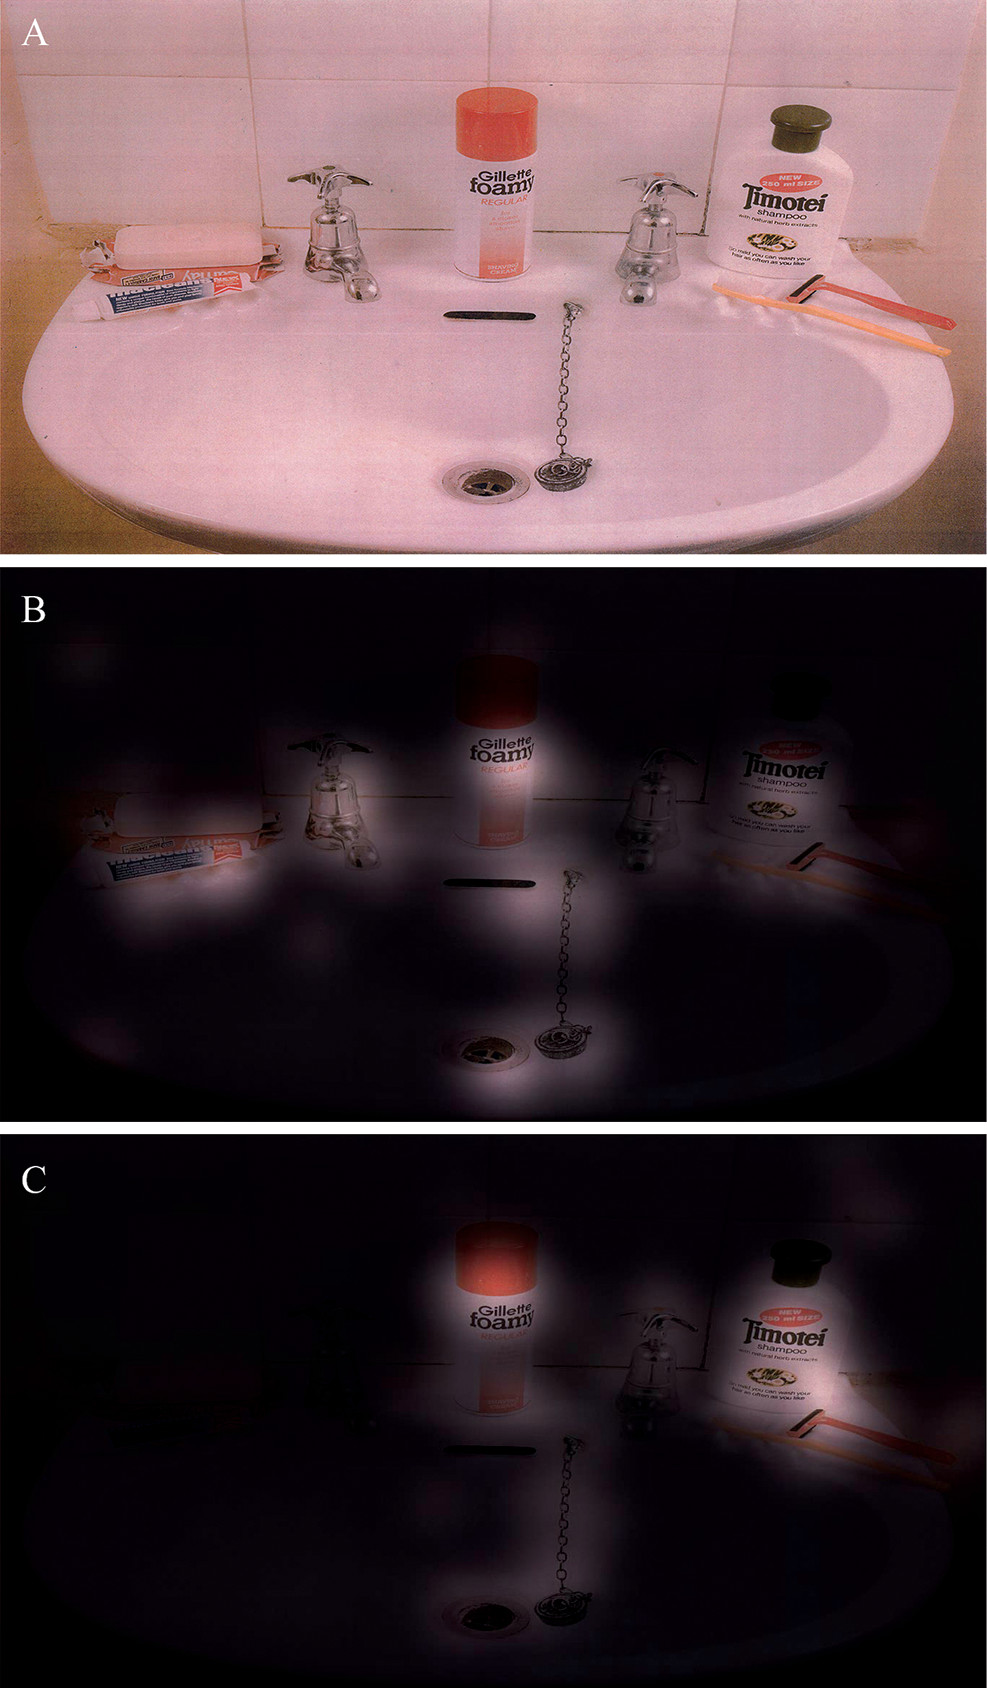
\includegraphics[width=0.75\textwidth]{fov}
  \caption[Field of view comparison.]{(A) Behavioral inattention test with a
    washbasin; (B) healthy participant response; (C) left-neglect
    response. [4]}
  \label{fig:fov}
\end{figure}

\autoref{fig:tasks} further illustrates patients’ reduced interaction with
their left side. In \autoref{fig:tasks}, it’s critical to note that patients
don’t entirely neglect one side. The clock in \autoref{fig:tasks}.C for example
has a left half and only lacks numbers on the left. This indicates that, while
patients are less aware of their left side, they aren’t entirely unaware, but
rather need reminders to interact with this neglected side.

\begin{figure}[h]
  \centering
  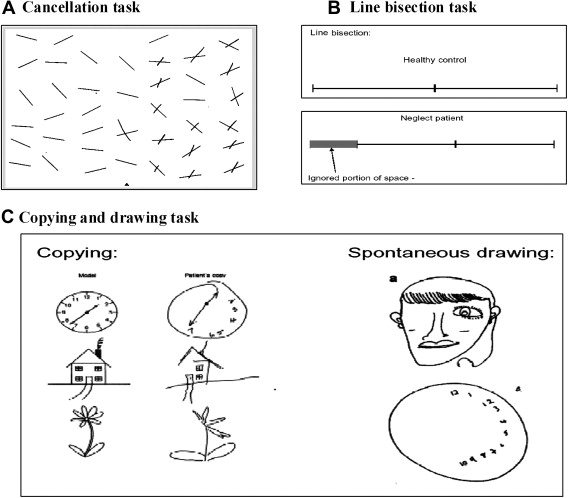
\includegraphics[width=0.65\textwidth]{tasks}
  \caption{Diagram depicting patient interaction with their left and right
    sides. [3]}
  \label{fig:tasks}
\end{figure}

However, this still depicts reduced interaction. When doing less-trivial tasks,
such as eating, this reduced interaction leads to immense struggle with common
daily tasks such as only eating the right half of one’s food, shown in
\autoref{fig:pasta}.

\begin{figure}[h]
  \centering
  
\includegraphics[width=0.65\textwidth]{pasta}
  \caption{Patients with left neglect may only eat the right half of their food
    [5].}
  \label{fig:pasta}
\end{figure}

\subsection{Types of Left Neglect}

The types of neglect faced by those with left USN can be broadly split into
four groups of neglect: personal, peripersonal, extrapersonal, and
temporal. The first three are defined by Ting et. al. and the last is defined
by Saj et. al. 

\subsubsection{Personal Neglect}

Personal neglect refers to neglect of one’s personal space, which literature
exemplifies with ``combing, grooming, shaving, recognizing the right half of the
body only'' and ``anosognosia'', or when patients are unable to recognize their
own disorder [3].

\subsubsection{Peripersonal neglect}

Peripersonal neglect is neglect of one’s peripersonal space (space which can be
immediately grasped) and includes ``eating food from the right half of the plate
and neglecting the food on the left'' and ``reading the right half of the two
pages of an open book'' [3]. \autoref{fig:pasta} is an example of peripersonal
neglect.

\subsubsection{Extrapersonal neglect}

Extrapersonal neglect is neglect of one’s extrapersonal space (space beyond
one’s arm’s reach) and includes failure to identify people on the left or
collision with objects on the left [3].

\subsubsection{Temporal neglect}

Unlike the previous three categories, temporal neglect is a non-physical
category of neglect. Research [6] describes that those with left spatial
neglect are less able to perceive the past, which is the ``left [side] [of] a
mental timeline.'' \autoref{fig:recall}, below, plots the proportion of events patients were
able to correctly associate with ``past'' or ``future''; there is a substantial
difference for patients with left spatial neglect who are more likely to
associate past events as future and vice versa.

\begin{figure}[h]
  \centering
  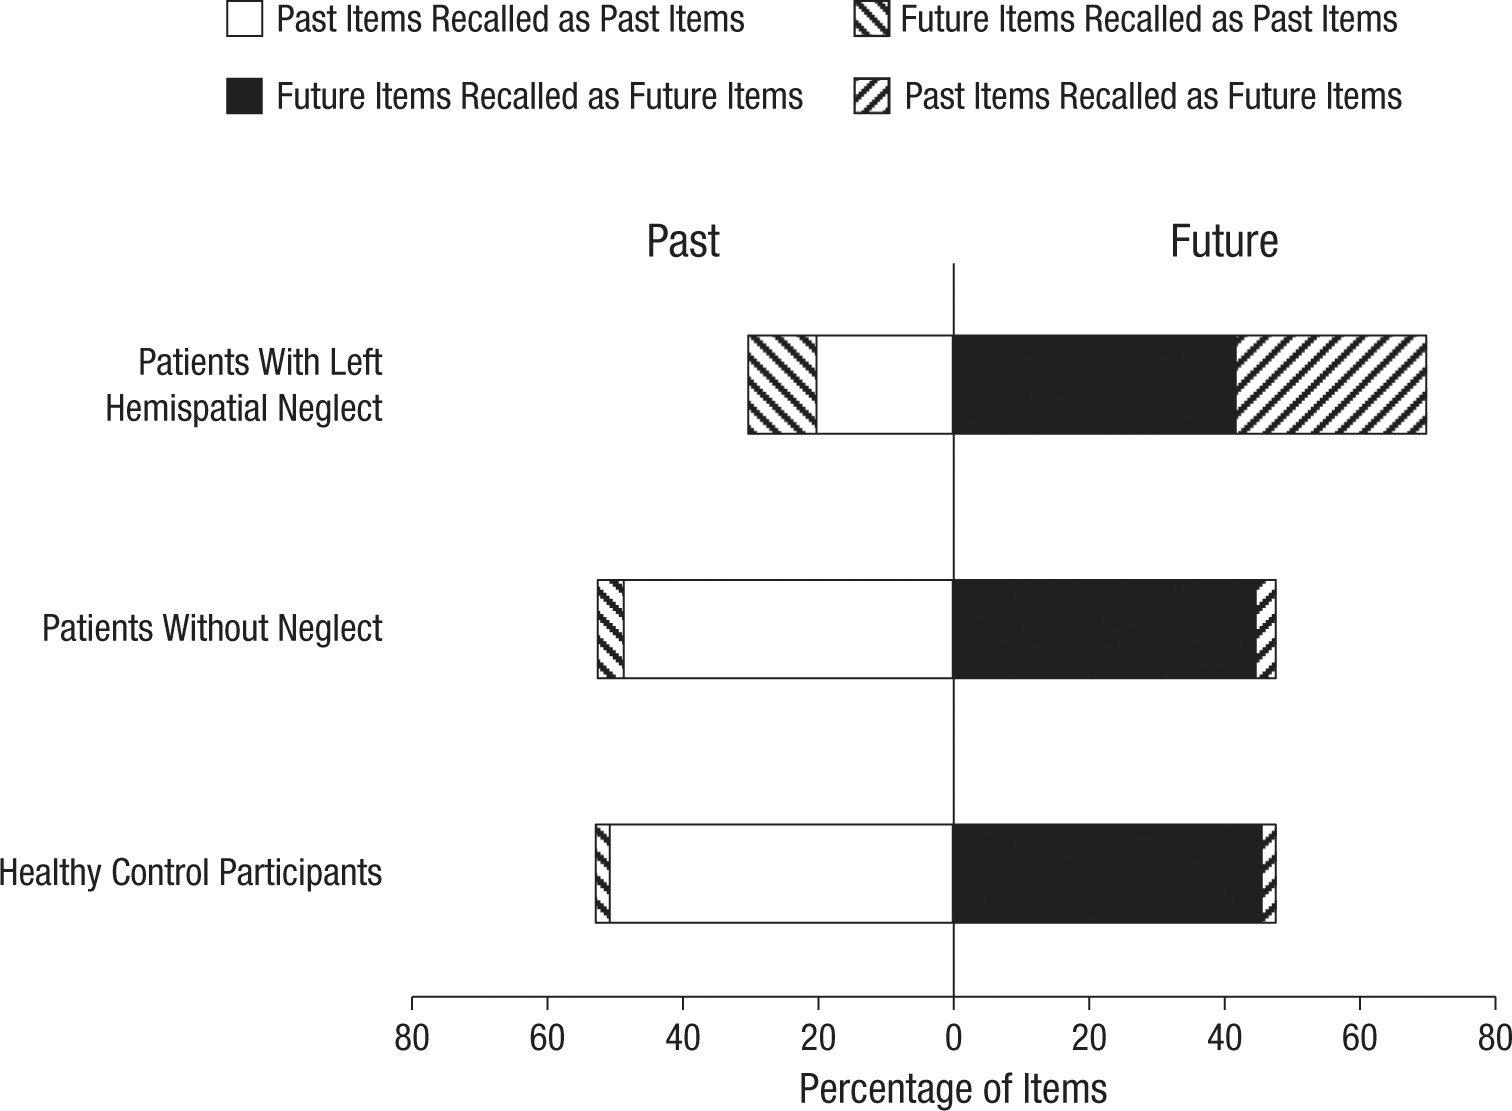
\includegraphics[width=0.75\textwidth]{recall}
  \caption{Temporal neglect of patients with left spatial neglect quantified by
    percentage of items correctly recalled.}
  \label{fig:recall}
\end{figure}

Research describes that this existence of temporal neglect implies that time
has spatial properties [6]. More importantly, this type of neglect gives
interesting insight when it comes to types of neglect faced by those with
unilateral spatial neglect: not all types of neglect are physical, meaning even
if a design idea could perfectly solve the physical aspects of neglect, it
would not be 100\% effective at solving all aspects of neglect.

\section{Reviewing current approaches to left neglect}

Current approaches to left neglect are extensive with multiple patented
commercial products. Here, two specific therapies are explained in detail.

\subsection{Specific Solution 1: Prism Adaptation}

Prism adaptation treatment is a process in which individuals wear prisms that
displace their vision in a specific direction while performing specific
direction-related tasks [7]. While research indicates that individuals
initially make errors, with repeated trials, the amount of errors decreases
[7]. This same research further explains that for those with left neglect,
right-shifting prisms shifts movement leftward [7] which directly tackles
aforementioned issues regarding personal, peripersonal, and extrapersonal
space. However, this solution is unlikely to alleviate temporal neglect due to
time not being physical. An ideal solution would provide means to alleviate
temporal neglect, though this necessarily complicates the design process by
involving both physical and non-physical categories of neglect.

\subsection{Specific Solution 2: “Visual Attention Therapy” App}

\autoref{fig:tasks2} summarizes how the “Visual Attention Therapy” (VAT) App
works. When an individual uses this app, they go through a timed trial in which
they interact with certain elements spread across an entire tablet screen
(A). At the end of the trial, individuals get results indicating where on the
screen they were more likely to neglect (B). This information can be used to
reduce the number of missed targets by giving individuals instant feedback.

\begin{figure}[h]
  \centering
  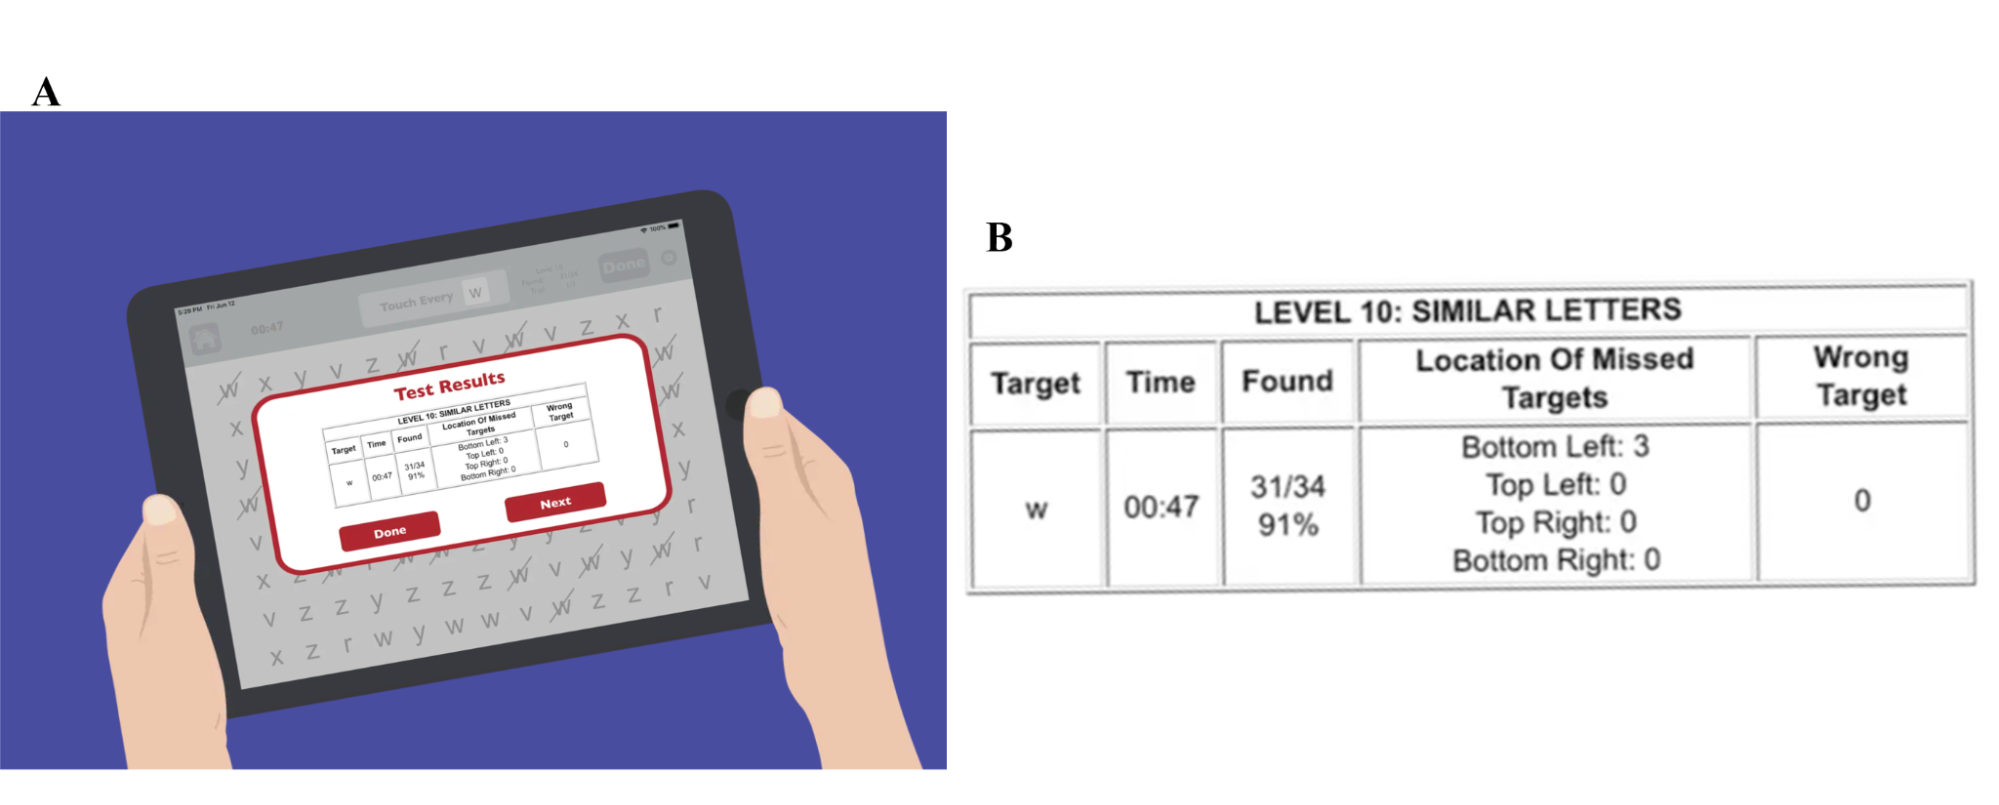
\includegraphics[width=\textwidth]{tasks2}
  \caption[VAT App.]{(A) Screenshot of VAT App from official website [8]; (B)
    zoomed in screenshot of test results page which indicates location of
    missed targets.}
  \label{fig:tasks2}
\end{figure}

\subsection{Review of Therapies}

Both of these therapies share one flaw: individuals cannot use them at any
time, as they have to be in a comfortable, safe environment, meaning this
solution is unable to help people when they may need it in public. The prism
device is designed to only be worn for 20 or so minutes at a time [7], multiple
times per week – literature indicates that at least twice per week prism device
usage is needed for rehabilitative effects [7]. The app requires using an
electronic device, constraining it to use only where and when an electronic
device can be used.

\section{Conclusion}
Left neglect, a subset of unilateral spatial neglect, leads to deficiencies in
interaction in affected individuals in multiple categories. These deficiencies
decrease individuals’ ability to fully interact with their world. Current
solutions for left neglect are used in therapy; the two cited are both good
examples, but are also restrictive in use cases. Neglect faced by affected
individuals reduces quality of life, meaning a general solution for either left
or right unilateral spatial neglect would be a critical tool in improving
quality of life for affected individuals. However, as indicated in Figure 1,
the relative severity of right-side USN makes designing an assistive device for
left-side USN both more feasible given time constraints and necessary given its
prevalence.

%%% Local Variables:
%%% mode: latex
%%% TeX-master: "../final_report"
%%% End:
